\documentclass {article}
\usepackage{fullpage}

\usepackage{graphicx}

\begin{document}

~\vfill
\begin{center}
\Large

A5 Project Report

Title: Space Wandering

Name: Joseph Reusing

Student ID: 20521843

User ID: jrreusin
\end{center}
\vfill ~\vfill~


\newpage
\section{Table of Contents}
\tableofcontents



%%%%%%%%%%%%%%%%%%%%%%%%%%%%%%%%%%%%%%%%%%%%%%%%
% OBJECTIVES
%%%%%%%%%%%%%%%%%%%%%%%%%%%%%%%%%%%%%%%%%%%%%%%%
\newpage
\section{Objectives}
\textbf{Full UserID: jrreusin\\Student ID: 20521843}
\begin{enumerate}
     \item[\_\_\_ 1:]  Objective one. Modelling a spaceship and obstacles (asteroids and comets).

     \item[\_\_\_ 2:]  Objective two. UI to display points earned in the game and to toggle graphical options.

     \item[\_\_\_ 3:]  Objective three. Texture Mapping to map realistic textures to each of the models.

     \item[\_\_\_ 4:]  Objective four. Bump mapping on the asteroids and comets to create craters and other imperfections.

     \item[\_\_\_ 5:]  Objective five. Reflection mapping on parts of the spaceship to give a metallic effect.

     \item[\_\_\_ 6:]  Objective six. Detect collision between the spaceship and asteroids and comets using Axis Aligned Bounding Boxes (AABB).     
     
     \item[\_\_\_ 7:]  Objective seven. Utilize particle systems to create an explosion effect (upon collision).

     \item[\_\_\_ 8:]  Objective eight. Sound effect synchronization of collisions and lasers shooting.
     
     \item[\_\_\_ 9:]  Objective nine. Lens flares when the main light source passes across the screen/camera.

     \item[\_\_\_ 10:] Objective ten. Make cel shading an available option for a different look to the game.
     
\end{enumerate}

Note: Only objectives 1-5 were completed. Incomplete implementations of objectives 6 and 7 will be described later but are not functional.


%%%%%%%%%%%%%%%%%%%%%%%%%%%%%%%%%%%%%%%%%%%%%%%%
% PROJECT INFO AND GOALS
%%%%%%%%%%%%%%%%%%%%%%%%%%%%%%%%%%%%%%%%%%%%%%%%
\newpage
\section{Project Information and Goals}
\subsection{Purpose}
\hspace{0.5cm}This project will be an OpenGL space exploration game using where you move a spaceship in 3D space as you explore forward into the screen avoiding space obstacles (asteroids).
	
	The purpose of this project is to utilize a variety of graphics techniques in OpenGL to create a polished looking space exploration game.
	The techniques/objectives will be further detailed below.

\subsection{Statement}
%{\bf What it's about. }	
	
	\hspace{0.5cm}This game is about a space explorer controlling a spaceship in 3D space with a 3rd person view centered on the spaceship at all times. The player will use the arrow keys to rotate the spaceship and press the spacebar to propel forward into the screen.
	Space can be very dangerous filled with many obstacles. The player must either avoid these obstacles or shoot them with the ships built in lasers which will just shoot straight forward. The purpose of the game is to survive as long as possible while gaining as many points as possible (by destroying obstacles).
	
	%{\bf What to do. }
	
	Firstly, the models for the spaceship and obstacles need to be made. Texture mapping will be used to give each of the models colour. On top of the texture mapping, a bump mapping will be used to give the space rocks a realistic looking surface with craters and such.
	Static collision detection will be used to detect collisions between the spaceship and the obstacles.
	Particle systems will be used to create an exploding effect when destroying an enemy with the spaceship lasers or when the spaceship collides with an obstacle. 
	A skybox will be used to simulate a space environment along with a cube mapping to give each of the faces of the skybox a texture. 
	Reflection mapping will be done on the spaceship to give it a metallic reflective looking surface. It will also help to highlight the spaceship as the center of attention.
	Sound effects such as the spaceship engine and collisions/explosions will need to synchronized to the moment the spacebar is pressed or the collision occurs.
	Lens flares will be added to the game when the camera looks towards the sun to add realism to the game.
	Cel shading will also be used as a toggle-able effect to provide a different visual experience to the game.
	
	
	%{\bf Why it is interesting and challenging.}
	
	This is an interesting project since it provides many graphical techniques that are new to me. It is a fun challenge to figure out how to use things like bump mapping, particle systems, reflection mapping and more to create an immersive space game.
	

	%{\bf What I will learn. }
	
	I will learn how to create a beautiful looking space game with necessary game functionality such as collision detection and sound synchronization. Lens flares are also something that I've always thought was a cool effect in movies and photos so it will be interesting to learn how to generate the effect programatically. 
	Cel shading is also something that interests me as I have observed it in many different 3D games before (like The Legend of Zelda: The Wind Waker, Breath of the Wild and Okami) giving a cartoonish effect and I've always wanted to learn how it is done.


%%%%%%%%%%%%%%%%%%%%%%%%%%%%%%%%%%%%%%%%%%%%%%%%
% PROJECT MANUAL
%%%%%%%%%%%%%%%%%%%%%%%%%%%%%%%%%%%%%%%%%%%%%%%%
\newpage
\section{Project Manual}
\subsection{Compilation}
\hspace{0.5cm}My submission for this project is a compressed folder containing all my project code and assets. Before compiling the code, extract the folder and place it in the cs488 folder.\\

Follow these steps to compile all the necessary code:
\begin{itemize}
	\item[1.] Change to the c488 directory
	
	cd .../cs488
	\item[2.] Compile the libraries and the cs488-framework
	
	premake4 gmake\\make
	
	\item[3.] Change to the extracted folder directory
	
	cd .../Project\_Jrreusin
	
	\item[4.] Compile the Project
	
	premake4 gmake\\make
	
\end{itemize}
\subsection{Running the Game}
\hspace{0.5cm}To run the game, you simply need to pass one .lua argument to the A5 executable. This .lua file should contain the spaceship model (formatted in the same way as the A3 hierarchical .lua files). I recommend using my spaceship model by using the Assets/spaceship.lua file.\\

./A5 Assets/spaceship.lua

\subsection{Controls and Options}
\hspace{0.5cm}When you run the game, a spaceship will be rendered directly in front of the camera along with many asteroids (better known as cuberoids) randomly spawned around the spaceship.

The arrow keys rotate the camera and the spaceship around a point that is directly in front of the spaceship. The spacebar will start to accelerate the spaceship forward into the screen.

If you look at the menu bar at the top of the game, you will see an \textbf{options} dropdown menu. Here you can toggle the skybox visibility and enable/disable the bump/normal mapping on the asteroids.



%%%%%%%%%%%%%%%%%%%%%%%%%%%%%%%%%%%%%%%%%%%%%%%%
% IMPLEMENTATION
%%%%%%%%%%%%%%%%%%%%%%%%%%%%%%%%%%%%%%%%%%%%%%%%
\newpage
\section{Implementation}
\hspace{0.5cm}For this implementation section, I will describe how each objective was achieved and which pieces of code were relevant. Note that since I did not complete all of my objectives, I will only go into deep detail for the first 6 objectives. I will then briefly describe how I planned to implement the missing objectives in the last subsection.

\subsection{Modelling}

\hspace{0.5cm}The spaceship was modelled using the completed Assignment 3 code. It is a simple looking spacecraft made up of only scaled coloured cubes. The cube shaped asteroids are simply made from the cube.obj which is imported through the MeshConsolidator. 

The skybox is also a cube whose vertices are defined and buffered in the A5::uploadVertexDataToVbos() function.

\subsection{User Interface}
\hspace{0.5cm} The user interface is relatively simple mostly due to the incomplete objectives. Here are the following options graphical options I was able to include in the options menu:
	\begin{itemize}
  	
  		\item[1. ] Bump Map - This option toggles the bump/normal map. This option allows you to clearly see the difference between a diffuse texture by itself and a diffuse texture with a normal map.
  		\item[2. ] Skybox - this option toggles the rendering of the skybox. The skybox makes the environment seem much more realistic. It makes it feel like you are really in space with the high definition starry skybox. When disabling the skybox, you will see that the space effect is lost.
		\item[3. ] A3 Graphical options are also included: Toggle z-buffering, back-face culling and front-face culling 
	\end{itemize}

\begin{figure}[h]
\begin{center}
	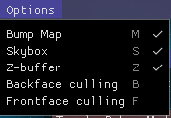
\includegraphics[width=0.3\textwidth]{optionsmenu.png}
	\caption{Graphical Options Menu}
  \label{fig:options}
\end{center}
\end{figure}


Finally there is an on screen display that shows the frame-rate and the speed of the spaceship. You can also press the Toggle Debug Mode to display co-ordinate information, as well as other parameter values such as yaw and pitch (which determine the camera/ship rotation).

\begin{figure}[h]
\begin{center}
	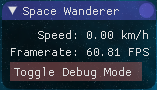
\includegraphics[width=0.2\textwidth]{onscreen.png}
	\caption{On Screen Display}
  \label{fig:onscreen}
\end{center}
\end{figure}

You can find all the UI implementation A5::guiLogic() in the A5.cpp file.

\subsection{Texture Mapping}
\hspace{0.5cm}There are 2 main texture assets used in this project: the skybox texture (6 different .png files for each face of the skybox) and the asteroid diffuse map texture. 

\subsubsection{Skybox Texture}
\hspace{0.5cm}In the A5::init() function, you can see in the shader configuration section, the skybox shader samplerCube is set to 0. Also in this function, we can see a call to A5::loadCubeMap();
which generates an OpenGL CubeMap Texture and loads each of the 6 images (stored in the Assets/lightblue folder) for the skybox to the texture. It then returns the textureID so that we can use the texture later.

In the A5::draw() function, you can see a call to the A5::renderSkybox() function which will bind the cubemap texture and draws the skybox triangle vertices using the vao\_skybox global variable.

\begin{figure}[h]
\begin{center}
	\includegraphics[width=0.3\textwidth]{cubemap.png}
	\caption{Cube Map Textures.}
  \label{fig:cubemap}
\end{center}
\end{figure}

\subsubsection{Asteroid Texture}
\hspace{0.5cm} Similarily to the skybox texture, the diffuse map sampler2D in the normal\_map\_shader is set to 0 in the shader configuration section in the init function. We also load the diffuse texture by making a call to the function loadJPEGTexture(``Assets/asteroid\_diffuse\_map.jpg").

In the A5::draw() function, we make a call to the A5::renderAsteroids() which iterates through the asteroids vector that stores all the randomly generated asteroids. The vector contains Asteroid object instances which is defined in the Asteroid.hpp and Asteroid.cpp. The Asteroid object contains information like position, transformation, direction and speed.
For each Asteroid, we call A5::renderCube(mat4 trans, mat4 pos) where we pass the transformation and position from the Asteroid object. The diffuse map texture is bound to GL\_TEXTURE0 and the cube vertices are drawn (which are loaded from the mesh consolidator into the buffer in A5::uploadVertexDataToVbos()).

\begin{figure}[h]
\begin{center}
	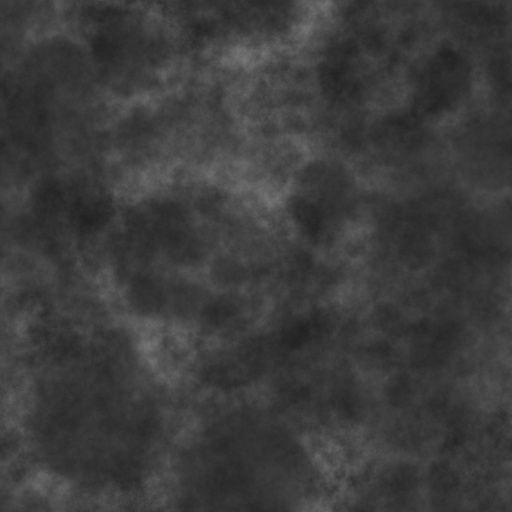
\includegraphics[width=0.23\textwidth]{asteroid_diffuse_map.jpg}
	\caption{Asteroid Diffuse Map}
  \label{fig:diffmap}
\end{center}
\end{figure}

\subsection{Bump/Normal Mapping}

\hspace{0.5cm} The normal/bump mapping is done along side the diffuse texture mapping as mentioned in the previous section. In the A5::init() function, we can see another call to the function 
loadJPEGTexture(``Assets/asteroid\_norm\_map.jpg"). Also note that the normal map sampler2D in the normal\_map\_shader is set to 1 in the shader configuration section in the init function.

In A5::renderCube the normal map texture is bound to GL\_TEXTURE1 before the cube vertices are drawn. The normal map represents each normal at each pixel with an RGB value that corresponds to the XYZ values for the normal vector. Knowing these vectors, we can render detailed surfaces on the cube asteroids.

\begin{figure}[h]
\begin{center}
	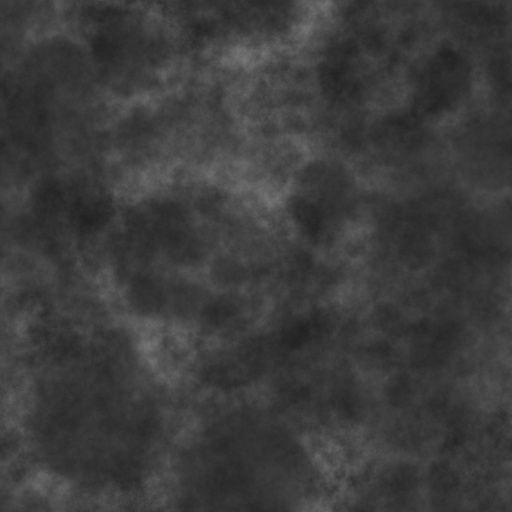
\includegraphics[width=0.3\textwidth]{asteroid_diffuse_map.jpg}
	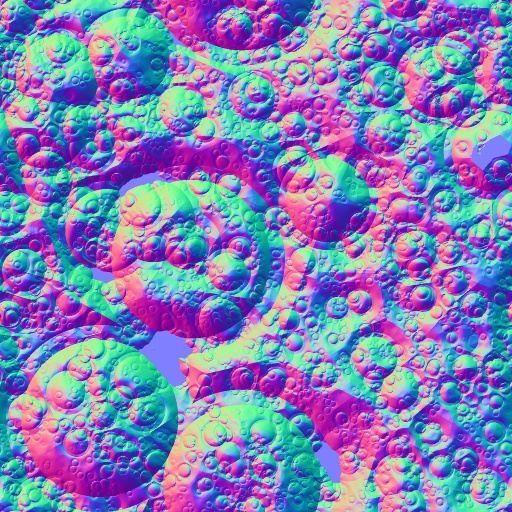
\includegraphics[width=0.3\textwidth]{asteroid_norm_map.jpg}
	\caption{Diffuse Map and Normal Map}
  \label{fig:normmap}
\end{center}
\end{figure}

Most of the normal mapping work is done in the normal map shader (find the shader code in ``normal\_map.vs" and ``normal\_map.fs"). Aside from positions and normals, we pass the Texture Coordinates, the tangents and bitangents (which are calculated and buffered in A5::uploadVertexDataToVbos()) to the shader. We use these values to build a TBN matrix (Tangent, Bitangent, Normal matrix) which we can use to get the LightPos, ViewPos (camera position), and fragment position in tangent space. These tangent space positions are passed to the fragment shader which are used to calculate the diffuse and specular values which are combined with the ambient value to get the correct fragment colour.


\begin{figure}[h]
\begin{center}
	\includegraphics[width=0.5\textwidth]{bumpmapped.png}
	\caption{Cubic Asteroid with Normal Mapping Enabled}
  \label{fig:bumpmap}
\end{center}
\end{figure}

\subsection{Reflection Mapping}
\hspace{0.5cm} The reflection mapping just utilizes the same cube map texture used for the skybox which was described in the texture mapping section (5.3). My first goal was to figure out how to make a ``mirror" cube (a cube that reflects the skybox). When you run the game, you will notice that there is a ``mirror" cube rendered directly behind the asteroid in front of the ship. This reflective cube uses the cubemaps shader (shader code in ``cubemaps.vs" and ``cubemaps.fs"). Similarly to the skybox shader, we set the samplerCube to the skybox texture in the fragment shader. In the fragment shader, we calculate the normalized incident ray I using the camera position and the fragment position. We then get the reflected ray R using the built in reflect function. Finally, set the fragment colour to the colour sampled from the skybox using R.

After implementing the ``mirror" cube, it was easy to add a partial reflection effect on the spaceship. This was done by adding the skybox samplerCube to the spaceship fragment shader (``FragmentShader.fs"). To get a partial reflection, we simply mixed the phong model colour (from A3 implemented in ``FragmentShader.fs") with the reflected colour. Notice the small artifacts on the ship in the figure below (rather than just a flat shaded colour), these are partial reflections of the skybox.


\begin{figure}[h]
\begin{center}
	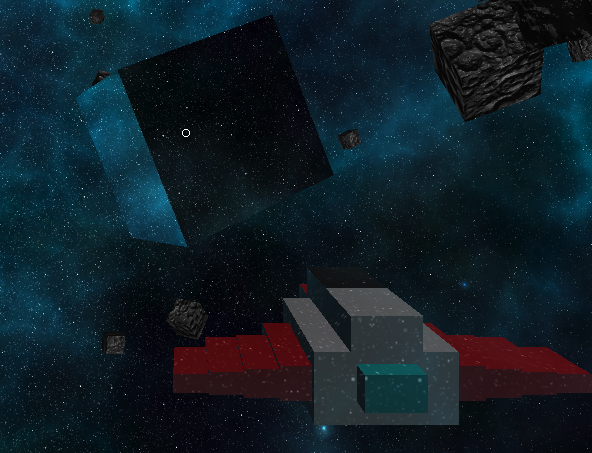
\includegraphics[width=0.5\textwidth]{reflect.png}
	\caption{Mirror Cube and Ship Reflections}
  \label{fig:bumpmap}
\end{center}
\end{figure}




\subsection{Partially Implemented Objectives}
\hspace{0.5cm}Sadly I was unable to complete all of the objectives and was only able to fully implement the first 5. I was able to partially implement AABB Collision detection and a Particle system but they are not functional. I will describe how I planned to have them working in this section.
\subsubsection{AABB Collision Detection}
\hspace{0.5cm}Axis Aligned Bounding Boxes or AABBs collision detection is a very nice  way to implement collision detection since you only need to keep track of 2 vertices for each bounding box. This is because an AABB can be represented by just the corner vertex with the smallest XYZ values and the corner vertex with the largest XYZ values. 

In this project, the AABBs are stored in a AABB class that is implemented in the files ``AABB.hpp" and ``AABB.cpp". Testing whether two AABBs are intersecting is implemented in the function AABB::Intersect(const AABB \&other) which just compares the distances of the min and max corners to check if the boxes are overlapping.

\subsubsection{Particle Systems}
\hspace{0.5cm}For particle systems, I planned to utilize the Particle structure I included in the A5.hpp file. The structure stored information position, velocity, colour and life. Each particle's values would be updated and re-rendered each frame.

The particles were to be rendered as quads always facing the camera. Sadly, I spent a large amount of time just trying to get a single one to render but I never found out the root issue since I ran out of time.


\subsection{Missing Objectives}
\hspace{0.5cm}I had always planned to finish all of the objectives at a bare minimum level but sadly I got stuck on the objectives mentioned above as I thought they were a higher priority than the ones missing.



%%%%%%%%%%%%%%%%%%%%%%%%%%%%%%%%%%%%%%%%%%%%%%%%
% CONCLUSIONS
%%%%%%%%%%%%%%%%%%%%%%%%%%%%%%%%%%%%%%%%%%%%%%%%
\newpage
\section{Conclusions}
\subsection{Lessons Learned}
\hspace{0.5cm}This may be an obvious lesson but for someone like me who struggles to manage his time well, implementing things in OpenGL can take a lot of time especially when you come across issues/bugs. I ended up spending loads of time trying to get my collision detection and particle systems to work correctly. In hindsight I should have probably moved on to other objectives since I could not figure out the problem(s) in the end.
\subsection{References}
	\begin{itemize}
  	
  		\item[1. ] {\bf OpenGL Programming Guide: The Official Guide to Learning OpenGL, Version 4.3 (8th Edition),} Schreiner et al., 2013, pp. 433 - 441 
  		\item[2. ] {\bf Computer Graphics with Open GL Fourth Edition,} Hearn, Baker and Carithers, 2014, pp. 545 - 562
  		\item[3. ]  {\bf The Cg Tutorial,} Fernando and Kilgard, 2007, ch. 07\\http://developer.download.nvidia.com/CgTutorial/cg\_tutorial\_chapter07.html
  		\item[4. ]  {\bf opengl-tutorial, } Chapter 18 - Particles/Instancing\\
     http://www.opengl-tutorial.org/intermediate-tutorials/billboards-particles/particles-instancing/
     
     	\item[5. ] {\bf Interactive Collision Detection for 3D Environments, } Mauro Figueiredo, 2013\\
     	https://pdfs.semanticscholar.org/0bb7/216bacac48a2a2d7fc5120425c8202f3fc93.pdf
     
	
	\end{itemize}

     






\end{document}
